% .:: Laden der LaTeX4EI Formelsammlungsvorlage
\documentclass[fs, footer]{latex4ei}

% Dokumentbeginn
% ======================================================================
\begin{document}


% Aufteilung in Spalten
\begin{multicols}{4}
	\fstitle{Technische \\ Mechanik}

\vspace{-2mm} % Man muss optimieren wos nur geht ;)

% ---------------------------------------
% | 		Mechanik					|
% ~~~~~~~~~~~~~~~~~~~~~~~~~~~~~~~~~~~~~~~
%=======================================================================



\section{Allgemeines}
%===================================================================
Skalar: $s$, Vektor: $\vec v$, Matrix: $\ma M$\\
%Modellierung: So genau wie nötig, so abstrakt wie möglich.\\
Innenwinkelsumme im $n$-Eck: $(n-2) \cdot 180^\circ$\\

\paragraph{Allg. Dreieck} $\triangle ABC$ mit Seiten $a,b,c$ und Winkel $\alpha,\beta,\gamma$:\\
Höhe: $h_c = a \sin \beta = b \sin \alpha$ \qquad Fläche $A = \frac{1}{2} h_c c$\\
Kosinussatz: \boxed{ c^2 = a^2 + b^2 + 2ab \cos(\gamma)}\\
Sinussatz: \boxed{\frac{a}{\sin \alpha} = \frac{b}{\sin \beta} = \frac{c}{\sin \gamma} = 2r}\\
Projektionssatz: $c = a \cos \beta + b \cos \alpha$\\ 
\\
Schwerpunkt: $x_S = \frac{1}{3}(x_A + x_B + x_C)$ \quad $y_S = \frac{1}{3}(y_A + y_B + y_C)$\\
\\
\paragraph{Rechtwinkliges Dreieck} $\triangle ABC$ mit $\gamma = 90^\circ$ bei $C$\\
Höhensatz: $h^2 = pq$ \quad Kathetensatz: $a^2 = pc$\\
\\
\emph{Grundformeln:}\\
	\begin{tabular}{l|l|l}
		Physikalische Größe & Translation & Rotation \\ \hline
		Strecke & $\vec x$ & $\vec \varphi = \vec x \cdot \frac{1}{r}$\\
		Geschwindigkeit & $\vec v = \dot{\vec x}$ & $\vec \omega = \dot{\vec \varphi}$ \\
		Beschleunigung & $\vec a = \dot{\vec v} = \ddot{\vec x}$ & $\vec \alpha = \dot{\vec \omega} = \ddot{\vec \varphi}$ \\
		Masse/Trägh. & $m$ & $\Theta = \int_V \vec r^2_\perp \diff m$ \\
		Impuls & $\vec p =m \vec v$ & $\vec L = \ma \Theta \vec \omega$ \\
		Kraft/Moment & $\vec F = \dot{\vec p} = m \vec a$ & $\vec M = \dot{\vec L} = \ma \Theta \vec \alpha$ \\
		Energie & $E_{kin}=\frac12mv^2$ & $E_{rot}=\frac12 \Theta \omega ^2$\\
		Leistung & $P = \vec F \bdot \vec v$ & $P = \vec M \bdot \vec \omega$\\
	\end{tabular}\\
Bewegungsgleichungen:\\
\boxed{\begin{array}{l}
	v=v_0 + at \\
	x(t)=\frac{1}{2}at^2+v_0t+x_0\\
	2ax=v^2-v_0^2 \end{array}}
\quad
\boxed{\begin{array}{l}
	\omega = \omega_0 + \alpha t \\
	\varphi(t)=\frac{1}{2}\alpha t^2+\omega_0t+\varphi_0\\
	2\alpha \varphi = \omega^2-\omega_0^2 \end{array}}\\
\\
\\
\emph{Newtonsche Gesetze:}\\
\begin{tabular}{ll}
	Trägheit & $m \vec v = \const$, falls $\sum \vec F = 0$\\
	Kinetik & $\sum F = \dot{ \vec p}$\\
	Gegenwirkung & actio = reactio\\
\end{tabular}\\
\\
\emph{Allgemeines Vorgehen:}
\begin{enumerate}\itemsep-2pt
	\item Welche Werte gegeben, welche kosntant, welche veränderlich?
	\item Geeignete Unterteilungen in Einzelsysteme
	\item Koordinatensysteme wählen
	\item Kräfte einzeichnen, Pfeilrichtung egal, VZ bestimmt phys. Richtung
\end{enumerate}
	
	\subsection{Drehmoment}
	\emph{Defnition:} Das Moment $M$ beschreibt die Drehwirkung, die eine Kraft $F$ aufgrund des Hebelarms $l$ auf einen Körper auszuüben versucht.\\ \\
	\begin{tabular}{ll|ll}
		3D  & $\vec M = \vec r_{OP} \times \vec F$ & 2D  &  $M = F \cdot l$ \\
	\end{tabular} \\ \\ 
	$\ra$ Das Drehmoment ist ein freier Vektor und kann beliebig verschoben werden.\\
	\paragraph{Kraftwinder} $(\vec F,\vec M)$: Paar aus Translationskraft und Drehmoment.\\
	Nullwinder $(0;0)$, Einzelkraft $(F;0)$, Einzelmoment $(0,M^P):$ \\


	\subsection{Statische GGW-Bedingung}
	\begin{tabular}{rl}
		$P$ & beliebiger Punkt \\
		$P_i$ &  Angriffspunkt für Einzelkräfte \\
		$\vec F_i$ &  Einzelkräfte \\
		$	\vec M_i$ &  Einzelmoment \\ 
		$\vec r_{PP_i}$ & Ortsvektor von $P$ nach $P_i$\\
	\end{tabular} \\ 
	\boxed{\sum \vec F = \vec 0}
	\boxed{ \sum \vec M^P = \vec 0 = \sum \vec M_j + \sum \vec r_{PP_i} \times \vec F_i}\\



	\subsection{Bauelemente}
	
		\paragraph{Seil}
		Überträgt nur Zugkräfte, vernachlässigtes Eigengewicht, infitisimale Krümmungsradien möglich.
		Reibungsfreie Umlenkung der Zugkraft möglich.

		\paragraph{Stab:}
		Überträgt Zug- und Druckkräfte in Stabrichtung.
		
		\paragraph{Balken} Stellvertretend für alle 1D Bauelemente.\\
		Übertragung von Normalkraft(N): normal zur Schnittfläche\\
		Querkraft(Q): In der Schnittebene\\
		Biegemoment (M): Moment aus Schwerpunkt der Schnittfläche\\
		
		
	%\subsection{Lager}
	%\begin{tabular}{llcll}
	%	& Symbol & FG & Zwang & Wertigkeit\\
	%Loslager & & 2 & $\downarrow$ & 1\\
	%Festlager & & 1 & $\downarrow \ra$ & 2 \\
	%Einspannung & & 0 & $\curvearrowleft \downarrow \ra$ & 3\\
	%Gelenk && 1& $\rightarrow \downarrow$ & 2	
	%\end{tabular}


	\subsection{Koordinatensysteme}
	%===================================================================
	Vektor $\vec v$ zur Basis $B$\\
	$\vec v = (_B \vec e_x, {_B} \vec e_y, {_B} \vec e_z) \bdot {_B}\vec v = v_x {_B} \vec e_x +  v_y {_B} \vec e_y + v_z {_B} \vec e_z$\\
	
	\begin{tabular}{ll}
		$\vec e^B_i$ & Basisvektor von in $i$-Richtung\\
		$u_i$ & Koordinate in $i$-Richtung bezüglich $B$\\
		$u_i \vec e^B_i$ & $i$-Komponente
	\end{tabular}
	% Bild mit eingezeichneten Vektoren neben Tabelle
	
	Basistransformationsmatrix ${}_{\ma B} \ma T_{\ma A}$ von Basis $\ma A$ zur Basis $\ma B$:\\
	Spalten entsprechen Basisvektoren von $\ma A$ in $\ma B$ dargestellt
	
	
	\subsubsection{Basisdehung}
	Darstellung eines Vektors $_1 \vec a$ aus KOSY 1 in KOSY 2 \\
	\parbox{4.6cm}{
	\emph{Drehmatrix:}
	$\ma A_{21} = \mat{\cos \varphi & \sin \varphi & 0 \\ - \sin \varphi & \cos \varphi & 0 \\ 0 & 0 & 1}$ \\
	\emph{Rücktransformation:} $\ma A_{12} = \ma A_{21}^\top = \ma A_{21}^{-1}$
	}
	\parbox{2.2cm}{
		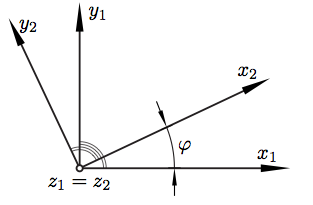
\includegraphics[width=2.2cm]{./img/Drehung-KOSY.png}		
	}	

	
	
	\subsection{Freiheitsgrade}
	Anzahl von unabhängigen Koordinaten um die Lage eines Körpers zu bestimmen.\\
	Punkt im Raum: 3(3 Lage), Körper im Raum: 6(3 Lage, 3 Winkel), Körper in der Ebene: 3(2 Lage, 1 Winkel)\\

	
	\subsection{Systemgrenzen}
	Zur Bestimmung von Reaktions und Schnittkräften wird das System in Teilsysteme zerlegt.
	Ist ein System im GGW sind es auch alle Teilsysteme.\\
	\\
	Freischnitt:\\
	\begin{enumerate}\itemsep0pt 
		\item KOSY wählen($x$ nach rechts, $z$ nach unten)
		\item gedachter, geschlossener Schnitt um jedes Element (keine Lager)
		\item Freistellen der Bauelemente
		\item Äußere (schon vorhandene) Kräfte eintragen.
		\item Für jede aufgetrennte Lagerbindung Reaktionskräfte einzeichnen:\\
				$\Ra$ pos. Wirkrichtung am pos. Schnittufer in pos. Richtung\\
				$\Ra$ neg. Schnittufer: Richtung nach Gegenwirkungsprinzip
		\item Einen beliebigen Punkt als Drehpunkt wählen
		\item Alle Momente bezüglich $P$ bestimmen, löse $\sum \vec M_i = 0$
	\end{enumerate}
	
	Konvention: Positive Schnittgrößen zeigen am positiven Schnittufer in positive Koordinatenrichtung.\\
	Tipp: Unbekannte Kräfte in positive Koordinatenrichtung antragen.\\
	

	\subsection{Innere Kräfte bestimmen}
	\begin{enumerate}
		\item Elemente bei Unstetigkeiten(Lager, Kräfte) in Bereiche teilen
		\item Pro Bereich einmal freischneiden und ein Schnittufer wählen
		\item Bestimme $N(x),Q(x),M(x)$ und löse GGW-Gleichungen
	\end{enumerate}
	Kräfteverteilung auf mehrere Lager: $\vec F_{max} \cdot (1-\frac{a}{l})$\\
	Diskrete Kräfte erzeugen\\ 
	Sprünge in $N(x)$ bzw $Q(x)$ bei paralleler Wirkrichtung\\
	Knicke in $M(x)$ wegen Sprung in $Q(x)$\\
	Sprünge in $M(x)$ bei Verzweigungen im Element\\
	
	
	
	\subsection{Kontinuierliche Kräfte }
	Streckenlast $q(x)$ (z.B. Eigengewicht) und $\diff F = q(x) \diff x$\\
	$\sum F = \int q(x) \diff x$ \qquad $\sum M^A = \int x q(x) \diff x$\\
	Resultierende Gesamtkraft $F_{res}$ darf nur zur Bestimmung der Lagerkräfte verwendet werden.



	%Bei Klausur: Wichtige Punkte einzeichen bringt bereits Punkte.
	
	\subsection{Lager}
	Verbindung eines Systems (z.B. Tragewerk) mit der Umwelt.\\
	Gewährleistung einer gewünschten Orientierung, Übertragung von Kräften.\\
	Lagerpunkte sind rotierbar.\\ \\
	\begin{tabular}{rl}
	Verschiebbare Lager (1-Wertig) & Rollenlager, Gleitlager, Pendelstütze\\
	Festlager (2-Wertig) &  Nur Drehung möglich.\\
	Feste Einspannung (3-Wertig) & Keine Bewegung möglich.\\
	Gelenk & Freie Rotation\\
	
	\end{tabular}	\\ \\
	\emph{kinematische Bestimmtheit: }  Wenn die Lagerung die Lage eines Körpers eindeutig festlegt (keine Bewegungsmöglichkeiten)\\
	\emph{statische Bestimmtheit: } Wenn die Lagerreaktionen eindeutig aus dem GGW bestimmt werden können\\ \\ 
	\parbox{4.6cm}{
	\begin{tabular}{rl}
	$f$ &  Freiheitsgrade \\
	$i$ & Anzahl der Körper \\
	$g$ & Freiheitsgrade d. ungebunden Körpers \\
	$k$ & Anzahl der Lager \\
	$W_n$ &  Wertigkeit des $n$-ten Lagers\\
	\end{tabular} }	
	\parbox{2.0cm}{\boxed{ f = g \cdot i - \sum\limits_{n=1}^k w_n }}
$\;$ \\ \\  \\ 
	\begin{tabular}{ll}
		$f=0$ & notwendige ,  n. hinreichende Bedingung für sta. Bestimmtheit.\\
		$f<0$ & System $|f|$-fach unbestimmt (Elastostatik)\\
		$f>0$ & System $f$-fach kinematisch überbestimmt (wackeliger Tisch)\\
	\end{tabular} \\ \\
	Drehgelenkt in der Ebene mit 3 Körpern: 4-wertig\\
	Drehgelenkt in der Ebene mit 2 Körpern: 2-wertig\\
	\fbox{Seilverankerungslager: Nur Einwertig!!!}
	
	
	\subsection{Schwerpunkt}
	ist der Bezugspunkt $S$, der in einem parallelen Kraftfeld $\Delta G$ immer den Kraftwinder $(G,0)$ ergibt. \\  \\ 
	$(\vec G,\vec 0) = \begin{cases} \vec G = \sum \Delta \vec G_i \\ \vec M^B = \sum (\vec r_{SP_i} \times \Delta \vec G) = \vec 0 \end{cases}$
	mit $\vec G = \sum \Delta G_i \vec e$\\ \\  \\ 
	\parbox{4.0cm}{
	$\sum \vec r_{SP_i} \cdot \Delta G_i = 0$\\ 
	$\int_K \vec r_{SP} \diff G = 0$} \parbox{2.5cm}{ \boxed{ m \vec r_{0S} = \int \vec r_{0P} \diff m }}
	\\
	Homogener Körper: $\vec r_{0S} = \frac{1}{V} \int_K \vec r_{0P} \diff V$\\
	Homogene Flächendichte: $\vec r_{0S} = \frac{1}{A} \int_K \vec r_{0P} \diff A$ (Dicke konst.)\\
	
	Allgemeine Formel: \boxed{\vec r_{0S} = \frac{\sum m_i \vec r_{0S_i}}{\sum m_i} }\\
	$\text{Schwerpunkt} = \frac{\text{Teilflächen} \cdot \text{Teil-Schwerpunkte}}{\text{Gesamtfläche}}$\\
	
	
	\subsection{Reibung}
	Rreibkegel: $\tan \delta_0 = \frac{F_{R,max}}{F_N} = \mu_0$\\
	\\
	Klotz auf schiefer Ebene:
	$\sum F_x = 0 = -F_R + m g \sin \beta$\\
	$\sum F_y = 0 = F_N - m g \cos \beta$\\
	\\
	Haftbedingung: $|F_R| \le \mu_0 F_N$ \quad $\Ra$ \quad $\tan \beta \le \mu_0$\\
	
	% Warum steht das hier 2x ?
	Vorgehen Gleitreibung:

	\begin{enumerate}
		\item Freischnitt
		\item Antragen der Normalkräfte als Druck- bzw. Reibkräfte entgegen Relativbewegung
		\item Aufstellen des Reibgesetzesb
		\item Bestimme unbekannte Kräfte
	\end{enumerate}

	Vorgehen Gleitreibung:
	\begin{enumerate}
		\item Freischnitt
		\item Antragen der Normalkräfte als Druck- bzw. Reibkräfte in pos. Richtung
		\item Aufstellen der GGW- und evtl. Kinematikbedingung
		\item Gültigkeitsprüfung des Reibgesetzes
	\end{enumerate}


\section{Stereo-Statik}
%===================================================================
Berechnung von äußeren und inneren Kräften auf ruhende, starre Körper und Punktmassen.\\
\\
\begin{tabular}{rl}
Wirklinie & Gerade entlang der Kraftrichtung.\\
Linienflüchtig & Vektor entlang der Wirklinie verschiebbar.\\
Angriffspunkt &  Punkt auf dem die Kraft wirkt. \\
Gleichgewicht & Körper in Ruhe und $\sum \vec F = 0$\\
Starrer Körper & Körper, der unter Einfluss von Kräften \\ &  keine Verformung erfährt. 
\end{tabular} \\ 

$\ra$ Der Abstand zweier Körperfester Punkte ist konstant.\\
Kräfte an einem starren Körper sind linienflüchtige Vektoren und können entlang ihrer Wirklinie verschoben werden. \\ \\
Arten von Kräften:
\begin{itemize}
\item Einzelkraft, Linienkraft, Flächenkraft, Volumenkraft \\
\item Normalkraft: Senkrechte Zwangskraft, die das durchdringen von Flächen verhindert.
\end{itemize}


\section{Elastostatik}
%===================================================================
Beanspruchung und temporäre Verformung von elastischen, statischen Bauteilen.


	\subsection{Spannung (Beanspruchung)}
	Spannung $\sigma(x) = \frac{\text{Kraft}}{\text{Fläche}} = \frac{F_N(x)}{A(x)}$ in $[\si{\newton \per \milli \meter^2}]$\\
	\\
	Normalspannung $\sigma = \frac{F_N \cos{\varphi}}{A}$\\
	Schubspannung $\tau = \frac{F_T \cos{\varphi}}{A}$\\

	Im geschnittenen Stab: $\sigma = \frac{F}{2A} (1 + \cos \varphi)$ \qquad $\tau = \frac{F}{2A} \sin (2 \varphi)$\\
	
	\subsection{Dehnung $\varepsilon$ (Verformung)}
	 
	Globale Dehnung $\varepsilon = \frac{\Delta l}{l}$ \\
	lokale Dehnung $\varepsilon(x) = \frac{\diff u}{\diff x}$
	Querdehnung: Poissonzahl: $\nu = - \frac{d}{\Delta d} \frac{\Delta l}{l}$\\
	\\
	Experimentelle Bestimmung über Zug-Druck-Versuch:\\
	Kraft anlegen, kontinuierliche Dehnungssteigerung, Messung der Spannung:\\
	Proportionalitätsgrenze $\sigma_p$, Fließspannung $\sigma_F$, Zugfestigkeit $sigma_m$\\
	\begin{tabular}{lll}
	I: & $0 \le \sigma \le \sigma_p$ & linear-elastischer Bereich\\
	II: & $\sigma \approx \sigma_F$ & plastischer Fließbereich\\
	III: & $\sigma_p \le \sigma \le \sigma_m$ & Verfestigungsbereich\\
	IV: & $\sigma_m \le \sigma$ & Einschnürungsbereich\\
	\end{tabular}
	
	Hookesches Gesetz: $\sigma = E \cdot \varepsilon_M$\\
	mit Elastizitätsmodul $E$
	
	\begin{tabular}{lll}
		Material & $E$ & $\alpha$ in $\SI{e-5}{\per \kelvin}$\\ 
		Stahl & $E = \SI{2.1e5}{\newton \per \milli \meter^2}$ & $1.2$\\
		Aluminium & $E_A = \SI{0.7e5}{\newton \per \milli \meter^2}$\\	
	\end{tabular}

	thermische Dehnung $\varepsilon_T = \alpha_T \cdot \Delta T$\\
	Wärmeausdehnungkoeffizient $\alpha_T$
	Dehnungsgesetz: $\varepsilon = \varepsilon_N + \varepsilon_T = \frac{\sigma}{E} + \alpha_T \cdot \Delta T$\\
	
	Stoffgesetz am Einzelstab: $\frac{\diff u}{\diff x} = \frac{N}{E \cdot A} + \alpha_T \cdot \Delta T$\\
	mit Schnittnormalkraft $N(x)$\\
	Längenänderung $\Delta l = \int_0^l \varepsilon(x) \diff x$\\
	Sonderfall Linearfeder $\Delta l = \frac{F \cdot l}{E \cdot A}$\\


	Vorgehen (statisch bestimmt):\\
	\begin{enumerate}
		\item Bestimmung der Normalkraft (Zug pos., Druck neg. VZ)
		\item Berechnung der Spannung aus der Belastung under die Dehnung aus dem Stoffgesetz
		\item Bestimmung der Verschiebung bzw. Längenänderung durch Integration
	\end{enumerate}
	(Temp. Änderung führ nur zu Dehnungsänderung)

	statisch unbestimmt:
	Elastizität, Spannung 
	Tempänderung führt zu zusätzlicher Spannung.

\section{Kinematik}
%===================================================================
Beschreibung von Bewegungen in Zeit und Raum ohne Berücksichtigung von Kräften.\\
\subsection{translation (Verschiebung)}
$x(t), v(t), a(t)$
\subsection{Rotation (Drehung)}
Winkelgeschwindigkeitsvektor $\vec \omega$ ist ein freier Vektor. (Alle Punkte haben selbes $\omega$)\\
Drehachsenreihenfolge darf nicht vertauscht werden! \\
starrer Körper: $\vec \omega$ überall gleich: $\vec v_Q = \vec v_P + \vec \omega \times \vec r_{PQ}$\\
Momentanpol: Jede translation kann als rotation um fikiven MP beschrieben werden.\\
ideal abrollendes Rad: MP ist unten am Berührpunkt.\\
\boxed{v_i = \omega \cdot r_i } \\
$\vec \omega = \dot{\vec \varphi}(t)$ \qquad $\vec v_i = \vec \omega \times \vec r_i$\\


Vorgehen für Momentanpol: \boxed{ \vec v_P \perp \vec r_{MP,P} }
\begin{enumerate}
	\item Fixe MP suchen\\
		Festlager, Abrollendes Rad
	\item Fixe Geschwindigkeiten suchen
		Loslager, Gleiten
	\item Schnittpunkt von Polstrahlen zweier fester Körper = MP
	\item Gelenke gemeinsamer Punkte zweier Körper\\
	$\Ra$ gleiche Geschwindigkeit 
\end{enumerate}



\subsection{Relativkinematik}
Darstellung von Ort, Kraft und Momenten in beliebigen KOSY (inertial/beschleunigt)\\
${}_K \vec r_{PA}$ im bewegten  KOSY $K$ und ${}_I \vec r_{0P}$ im Inertialsystem $I$\\
${}_I \vec r_{PA} = {}_I \vec e^K_x {}_K x^* + {}_I \vec e^K_y {}_K y^*$\\
${}_I \vec r_{PA} = {}_I \ma T_K \cdot ({}_K x^*, {}_K y^*, {}_K z^*)^\top$\\
Trafomatrix ${}_I \ma T_K$ besteht aus Einheitsvektoren von $K$ in $I$ dargestellt.\\
${}_K \ma T_I = {}_I \ma T_K^{-1}$ falls Matrix orthogonal: ${}_I \ma T_K^{-1} = {}_I \ma T_K^\top$\\ 
\\
Drehreihenfolge:\\
$\ma A_{31} = \ma A_{32} \bdot \ma A_{21}$\\
Mathematische Operatoren von Vektoren sind nur bei gleicher Basis möglich!\\
\\
Zeitableitung:\\
Bei einem Vektor $\vec a$ in einem drehendem KOSY $K$ ist bei Zeitableitung die Produktregel zu beachten:\\
${}_K \vec a = \sum a_i \cdot {}_K \vec e_i \xrightarrow{\frac{\diff}{\diff t}} {}_K \dot {\vec a} = \sum \dot a_i \cdot {}_K \vec e_i + \sum a_i \cdot {}_K \dot {\vec e}_i$\\

Eulerformel: ${}_K \dot {\vec a} = {}_K \overset{\circ}{\vec a} + {}_K \vec \omega_K \times {}_K \vec a$\\
${}_K \vec \omega_K$: Absolute Winkelgeschw. vom KOSY $K$ im KOSY $I$ in $K$-Koordinaten ausgedrückt.\\
Geschwindigkeit:
${}_K \vec v_A = {}_K \dot {\vec r}_{0A} = {}_K \overset{\circ}{\vec r}_{0A} + {}_K \vec \omega_K \times {}_K \vec r_{0A}$\\
% ${}_K \vec v_A = {}_K \dot {\vec r}_{0A} = \underbrace{ {}_K \overset{\circ}{\vec r}_{0A} }_{\pbox{2cm}{\text{\tiny Komponentenweise} \\ \text{\tiny Ableitung}}} + {}_K \vec \omega_K \times {}_K \vec r_{0A}$\\
\\
Beschleunigung:
${}_K \vec a_A = {}_K \dot {\vec v}_{A} = {}_K \overset{\circ}{\vec v}_{A} + {}_K \vec \omega_K \times {}_K \vec v_{A}$\\
\\
Bewegung von Kolben $D$ über drehenden Angriffspunkt $C$ mit Hebelarm $DC$:\\
$\vec v_D = \vec v_{C} + \vec \omega \times \vec r_{CD}$\\


















% E-Techniker sind bessere Mathematiker als Maschinenbauer, zugegeben am 15.06.12 von Bastian Esefeld!






\section{Kinetik}
%===================================================================
Zusammenwirken von Kräften und Bewegungen und Bestimmung von Translation.\\
Impulssatz: \boxed{\vec{\dot p} = \frac{\diff}{\diff t} (m \vec v) = \sum \diff F_i = \vec F = m \vec a }\\
Drallsatz: \boxed{\vec{\dot L} = \frac{\diff}{\diff t} (\Theta \vec \omega) = \sum \diff M_i = \vec M = \Theta \vec \alpha  }\\
\\
Impuls $\diff \vec p = \vec v_p \diff m = \frac{\diff \vec r}{\diff t} \diff m$\\
$\vec p = \int_K \diff \vec p$\\
$\vec p = m \cdot \vec v_s$ \quad $[p] = \si{kg m \per s}$\\
\\
Impulssatz für $\diff m$: \boxed{\frac{\diff }{\diff t} \diff \vec p = \frac{\diff}{\diff t}(\vec v \diff m) = \diff \vec F}\\ 
$\frac{\diff }{\diff t} \vec p = \int_K \frac{\diff }{\diff t}(\vec v \diff m) = \frac{\diff }{\diff t}(m \vec v_s) = \vec F$\\
Für konstante Masse: $m \cdot \vec a = \vec F$\\

Impulserhaltung: Bei Abwesenheit äußerer Kräfte $\vec F$ bleibt der Impuls $\vec p$ eines abgeschlossenen Systems konstant


Trägheitstensor: ${}_K \ma \Theta^p = \mat{\Theta_{xx} & -\Theta_{xy} & -\Theta_{xz} \\ -\Theta_{yx} & \Theta_{yy} & -\Theta_{yz} \\ -\Theta_{xz} & -\Theta_{yz} & \Theta_{zz} }$ \quad ist sym.\\
Hauptdiagonale: Massenträgheitsmomente (MTM): $\Theta_{xx} = \int_K y^2 + z^2 \diff m$\\
Nebendiagonale: Massendeviationsmomente (MDM): 
$[\Theta_{ji}] = \SI{1}{\kilogram \meter^2}$\\
\\
Änderung des Bezugssystems:\\
${}_K \ma \Theta^p = \mat{\Theta_{xx} + (b^2 + c^2)m & & \\ -\Theta_{xy} + abm & \Theta_{yy} + (a^2 + c^2)m & \\ -\Theta_{xz} + acm & -\Theta_{yz} + bcm & \Theta_{zz} + (a^2 + b^2)m }$\\
$\theta, \Theta, \vartheta$
\\
Drall bzw. Drehimpuls von $\diff m$: $\vec L = \vec r \times \vec p$\\
Drall eines Körpers bezüglich Schwerpunkt $S$:\\
${}_K \vec L ^s = \int_K ({}_K \vec r_{SP} \times {}_K \vec v_{SP}) \diff m = {}_K \Theta^s \cdot {}_K \vec \omega$ \\
$[\vec L] = \si{\kilogram \meter^2 \per second}$


Ideal abrollende Walze = kein Schlupf = Haftreibung

Vorgehen zum Lösen Drall:
\begin{enumerate}
	\item Einführung geeigneter Koordinatensysteme
	\item Freischnitt aller Körper und Eintrag aller Schnittreaktionen
	\item Aufstellen der absoluten (Winkel-) Beschleunigung aller Körper
	\item Bestimmung der Trägheitsmomente / -tensoren der körper
	\item Aufstellen von Impuls- und Drallsätzen\\
		Impuls im Inertialsystem und Drall in Körperfesten KOSYs
	\item Kopplung über Kinematik und Schnittreaktionen
\end{enumerate}
Impusl: $(m \vec v)^K = \sum \vec F$ \qquad Drall $(\Theta \omega)^K = \sum \vec M$\\

\section{Energie}
$\diff E = \frac{1}{2} \vec v \vec v^\top \diff m = \frac{1}{2} v^2 \diff m$\\
\\
\boxed{T = }
$Q$ = Schwerpunkt $S$: $T = \frac{1}{2} m \vec v_S^2 + \frac{1}{2} \vec \omega^top \Theta^S \vec \omega$\\
$Q$ = Momentanpol $M$: $T = \frac{1}{2} \vec \omega^top \Theta^M \vec \omega$




In einem konservativen Kraftfeld $\vec F$ ist die verrichtete Arbeit $W$ zur Verschiebung eines Teilchens $m$ von $A$ nach $B$ wegunabhängig.\\
$\forall \vec r: \rot \vec F(\vec r) = 0$\\
Potentielle Energie $V$ ist ein Maß für die Fähigkeit einer konservativen Kraft $\vec F$ Arbeit $W$ zu leisten.\\

Arbeitssatz: $\Delta W = \Delta E$
$\diff \vec F \cdot \diff \vec r = \frac{\diff \vec v^\top}{\diff t}\diff m \diff$




% Ende der Spalten
\end{multicols}

% Dokumentende
% ======================================================================
\end{document}
